% Beamer presentation of partial results for Friday:
%   Part I : Ising coupling, conditional dynamics, Schur dephasing, and Bell-state obstruction
%   Part II: Exact reduced map vs. canonical master equation, numerical observation,
%            where large rates come from, degeneracy hypothesis, two-level model, and run comparison
%   Appendix: canonical-form derivation, blow-up vs. finite peaks, and ongoing analysis (A.1--A.9)
% Shares references.bib and notation with main_report.tex and main_beamer.tex.
% Build from reports/:
%   pdflatex -synctex=1 -interaction=nonstopmode -halt-on-error friday_beamer.tex
%   bibtex friday_beamer
%   pdflatex -synctex=1 -interaction=nonstopmode -halt-on-error friday_beamer.tex
%   pdflatex -synctex=1 -interaction=nonstopmode -halt-on-error friday_beamer.tex
\documentclass[aspectratio=169,11pt]{beamer}
\usepackage[T1]{fontenc}
\usepackage[utf8]{inputenc}
\usepackage{lmodern}
\usepackage{graphicx}
\graphicspath{{./}{reports/}{Figures/}{reports/Figures/}}
\usepackage{amsmath,amssymb,mathtools,booktabs,array}
\usepackage[numbers,sort&compress]{natbib}
\renewcommand{\bibsection}{}
\providecommand{\doi}[1]{\href{https://doi.org/#1}{\nolinkurl{doi:#1}}}

\definecolor{ink}{RGB}{25,43,60}
\definecolor{accent}{RGB}{0,110,125}
\definecolor{muted}{RGB}{95,110,125}
\setbeamercolor{normal text}{fg=ink,bg=white}
\setbeamercolor{structure}{fg=accent}
\setbeamercolor{frametitle}{fg=accent}
\setbeamertemplate{navigation symbols}{}
\setbeamertemplate{bibliography item}[text]
\setbeamertemplate{footline}[frame number]
\setbeamersize{text margin left=8mm,text margin right=8mm}
\setbeamertemplate{itemize item}{\small$\bullet$}

\newcommand{\ket}[1]{\lvert #1\rangle}
\newcommand{\bra}[1]{\langle #1\rvert}
\newcommand{\Tr}{\operatorname{Tr}}
\newcommand{\id}{\mathrm{id}}
\newcommand{\diag}{\operatorname{diag}}
\newcommand{\rank}{\operatorname{rank}}
\newcommand{\spec}{\operatorname{spec}}
\newcommand{\ZZ}{\mathrm{ZZ}}
\newcommand{\dmat}{\mathsf d}
\newcommand{\Heff}{H_{\mathrm{eff}}}
\newcommand{\appref}[1]{{\color{muted}\footnotesize Full derivation: Appendix, #1.}}
\newcommand{\ongoing}{{\color{muted}\footnotesize Ongoing analysis.}}

\title{Two edge spins with Ising coupling to an XXZ bulk}
\subtitle{Partial results: Bell-state no-go and the canonical master equation --- why the initial bulk state matters}
\author{Spin transport project}
\date{20 November 2026}

\begin{document}

\begin{frame}[plain]
\titlepage
\end{frame}

% ==============================================================
\section{Model and Bell-state obstruction}
% ==============================================================

\begin{frame}{Setup: Ising-coupled edge spins on an XXZ chain}
\small
Two spin-$1/2$ edge probes, $A$ and $B$, couple via $S^z S^z$ contacts to opposite ends ($1$ and $N$) of an $N$-spin XXZ bulk $E$ (order $A,1,\ldots,N,B$; Hilbert space $\mathcal H_{AB}\otimes\mathcal H_E$, $S^\alpha=\sigma^\alpha/2$, $\hbar=1$):
\begin{align*}
H_E&=J\sum_{j=1}^{N-1}\bigl(S_j^xS_{j+1}^x+S_j^yS_{j+1}^y+\Delta S_j^zS_{j+1}^z\bigr)\quad(\text{plus optional bulk boundary fields on }1,N),\\[-2pt]
V_{\ZZ}&=g_A S_A^zS_1^z+g_B S_N^zS_B^z,\qquad H^{(\ZZ)}=H_E+V_{\ZZ}.
\end{align*}
\begin{itemize}\setlength\itemsep{4pt}
\item Basis: $\ket0=\ket\uparrow$, $\ket1=\ket\downarrow$, edge computational basis $(\ket{00},\ket{01},\ket{10},\ket{11})$.
\item Uncorrelated preparation with \textbf{arbitrary} initial bulk state $\omega_E$ (pure $\ket{\psi_0}\bra{\psi_0}$ or mixed), $U_t=e^{-iH^{(\ZZ)}t}$:
\[
\rho_{ABE}(0)=\rho_{AB}(0)\otimes\omega_E,\qquad
\rho_{AB}(t)=\Lambda_t\bigl(\rho_{AB}(0)\bigr)=\Tr_E\bigl[U_t(\rho_{AB}(0)\otimes\omega_E)U_t^\dagger\bigr].
\]

\end{itemize}
\end{frame}

% ==============================================================
\begin{frame}{Conserved edge projections and four conditional bulk Hamiltonians}
\small
Both edge $z$-projections commute with the total Hamiltonian, $[H^{(\ZZ)},S_A^z]=[H^{(\ZZ)},S_B^z]=0$.
Label each edge configuration by $a=(s_A^a,s_B^a)\in\{00,01,10,11\}$ with $s_{A,B}^a=\pm\tfrac12$ and projector $P_a=\ket a\bra a$:
\[
H^{(\ZZ)}=\sum_{a}P_a\otimes H_a,\qquad
\boxed{U_t=\sum_{a}\ket a\bra a\otimes U_a(t),\qquad U_a(t)=e^{-iH_at}.}
\]
\begin{columns}[T,totalwidth=\textwidth]
\begin{column}{0.52\textwidth}
\[
\begin{array}{@{}c@{\quad}l@{}}
\toprule
\text{Edge } a & \text{Conditional bulk Hamiltonian } H_a\\\midrule
00 & H_E + \tfrac{g_A}{2}S_1^z + \tfrac{g_B}{2}S_N^z \\[2pt]
01 & H_E + \tfrac{g_A}{2}S_1^z - \tfrac{g_B}{2}S_N^z \\[2pt]
10 & H_E - \tfrac{g_A}{2}S_1^z + \tfrac{g_B}{2}S_N^z \\[2pt]
11 & H_E - \tfrac{g_A}{2}S_1^z - \tfrac{g_B}{2}S_N^z \\\bottomrule
\end{array}
\]
\end{column}
\begin{column}{0.45\textwidth}
\vspace{4pt}
\begin{itemize}\setlength\itemsep{5pt}
\item The four edge configurations define four invariant subspaces.
\item In each sector $a$, the bulk feels static longitudinal boundary fields $(\pm g_A/2,\,\pm g_B/2)$ at sites $1$ and $N$.
\item Exact for \emph{any} bulk Hamiltonian $H_E$ acting on $E$ alone.
\end{itemize}
\end{column}
\end{columns}
\end{frame}

% ==============================================================
\begin{frame}{Case I: Edge inputs $\ket{00},\ket{01},\ket{10},\ket{11}$ --- Full global evolution}
\small
Fix \emph{any} initial bulk state---pure $\ket{\psi_0}_E$ or mixed $\omega_E$---and prepare the edge spins individually in one computational state $\ket a\in\{\ket{00},\ket{01},\ket{10},\ket{11}\}$. Since $P_c\ket a=\delta_{ca}\ket a$, only \textbf{one branch} of $U_t$ acts:
\medskip
\begin{itemize}\setlength\itemsep{6pt}
\item \textbf{Pure bulk $\ket{\psi_0}_E$:} the four individual preparations evolve as
\begin{align*}
\ket{00}\otimes\ket{\psi_0}_E &\;\longmapsto\; \ket{00}\otimes e^{-iH_{00}t}\ket{\psi_0}_E, &
\ket{01}\otimes\ket{\psi_0}_E &\;\longmapsto\; \ket{01}\otimes e^{-iH_{01}t}\ket{\psi_0}_E,\\[2pt]
\ket{10}\otimes\ket{\psi_0}_E &\;\longmapsto\; \ket{10}\otimes e^{-iH_{10}t}\ket{\psi_0}_E, &
\ket{11}\otimes\ket{\psi_0}_E &\;\longmapsto\; \ket{11}\otimes e^{-iH_{11}t}\ket{\psi_0}_E.
\end{align*}
\item \textbf{Arbitrary bulk density matrix $\omega_E$ (pure or mixed):}
\[
\boxed{\rho_{ABE}^{(a)}(t)=U_t\bigl(\ket a\bra a\otimes\omega_E\bigr)U_t^\dagger
=\ket a\bra a\otimes\bigl(U_a(t)\,\omega_E\,U_a(t)^\dagger\bigr).}
\]
\item \textbf{Global structure:} the full state remains an \textbf{exact product across $A:B:E$} at all $t\ge0$. The bulk evolves nontrivially under $H_a$, while no edge spin flips and no probe--bulk entanglement is created.
\end{itemize}
\end{frame}

% ==============================================================
\begin{frame}{Case I: Edge inputs $\ket{00},\ket{01},\ket{10},\ket{11}$ --- Reduced density matrix}
\small
Tracing out the bulk $E$ from $\rho_{ABE}^{(a)}(t)=\ket a\bra a\otimes U_a(t)\omega_EU_a(t)^\dagger$ gives, by unitarity of $U_a(t)$ and $\Tr_E\omega_E=1$,
\[
\rho_{AB}^{(a)}(t)
=\ket a\bra a\,\underbrace{\Tr_E\bigl[U_a(t)\,\omega_E\,U_a(t)^\dagger\bigr]}_{=\,\Tr_E\omega_E\,=\,1}
=\ket a\bra a=\rho_{AB}^{(a)}(0).
\]
\begin{itemize}\setlength\itemsep{6pt}
\item Every computational basis state is an \textbf{exact stationary fixed point} of $\Lambda_t$ for all $t\ge0$ and every $\omega_E$:
\[
\boxed{\begin{aligned}
\Lambda_t(\ket{00}\bra{00})&=\ket{00}\bra{00}, &\qquad \Lambda_t(\ket{01}\bra{01})&=\ket{01}\bra{01},\\
\Lambda_t(\ket{10}\bra{10})&=\ket{10}\bra{10}, &\qquad \Lambda_t(\ket{11}\bra{11})&=\ket{11}\bra{11}.
\end{aligned}}
\]
\item Although each conditional bulk state $\omega_E^{(a)}(t)=U_a(t)\omega_EU_a(t)^\dagger$ depends on $a$ and $t$, a \emph{single} branch leaves no trace on $AB$ once $E$ is traced out ($U_a^\dagger U_a=I_E$).
\item By linearity, any incoherent mixture $\rho_{AB}(0)=\sum_a p_a\ket a\bra a$ is also completely frozen: $\rho_{AB}(t)=\rho_{AB}(0)$.
\end{itemize}
\end{frame}

% ==============================================================
\begin{frame}{Why $\ket{00},\ket{01},\ket{10},\ket{11}$ cannot generate a Bell state}
\small
Compare $\rho_{AB}^{(a)}(t)=\ket a\bra a$ with the four Bell states in the computational basis:
\[
\ket{\Phi^\pm}=\frac{\ket{00}\pm\ket{11}}{\sqrt2},\qquad
\ket{\Psi^\pm}=\frac{\ket{01}\pm\ket{10}}{\sqrt2}.
\]
\begin{itemize}\setlength\itemsep{6pt}
\item \textbf{1.\ Frozen populations (no spin exchange):}
$\ket{\Phi^\pm}$ requires diagonal $(\tfrac12,0,0,\tfrac12)$ and $\ket{\Psi^\pm}$ requires $(0,\tfrac12,\tfrac12,0)$. Under $V_{\ZZ}$, $[H^{(\ZZ)},S_{A,B}^z]=0$ forbids flip-flop transitions: population $1$ stays locked on $\ket a$.
\item \textbf{2.\ Zero off-diagonal coherence:}
Bell states require $\lvert\rho_{00,11}\rvert=\tfrac12$ or $\lvert\rho_{01,10}\rvert=\tfrac12$. Starting in a single branch $\ket a$, all twelve off-diagonal entries of $\rho_{AB}^{(a)}(t)$ remain identically zero.
\item \textbf{3.\ Zero entanglement for any bulk state:}
$\rho_{AB}^{(a)}(t)=\ket{s_A^a}\bra{s_A^a}\otimes\ket{s_B^a}\bra{s_B^a}$ stays a pure product state ($C(t)=0$, pure local marginals $\rho_A,\rho_B$ rather than $I_2/2$) for \emph{every} $\omega_E$, $H_E$, $g_{A,B}$, and $t$.
\end{itemize}
\medskip
\textbf{Consequence:} For the bulk to induce any nontrivial dynamics on $AB$, the initial edge state \emph{must already contain coherences} across multiple branches $a\ne b$. This motivates preparing $\ket{++}$.
\end{frame}

% ==============================================================
\begin{frame}{Case II: Starting in $\ket{++}$ --- Global and reduced evolution}
\small
Prepare $\ket{++}=\ket+_A\otimes\ket+_B=\tfrac12(\ket{00}+\ket{01}+\ket{10}+\ket{11})$, with uniform initial entries $(\ket{++}\bra{++})_{ab}=\tfrac14$.
\smallskip
\begin{itemize}\setlength\itemsep{5pt}
\item \textbf{Full global evolution:} all four conditional bulk evolutions run simultaneously in coherent superposition:
\begin{align*}
\text{Pure }\ket{\psi_0}_E:\quad &\ket{\Psi(t)}=\tfrac12\textstyle\sum_{a\in\{00,01,10,11\}}\ket a\otimes U_a(t)\ket{\psi_0}_E,\\[2pt]
\text{General }\omega_E:\quad &\rho_{ABE}(t)=\tfrac14\textstyle\sum_{a,b}\ket a\bra b\otimes U_a(t)\,\omega_E\,U_b(t)^\dagger.
\end{align*}
Diverging conditional bulk states $U_a(t)\ket{\psi_0}_E$ generally entangle the pair $AB$ with the bulk $E$.
\item \textbf{Reduced density matrix $\rho_f(t)=\Lambda_t(\ket{++}\bra{++})$:} tracing out $E$ compares distinct branches $a$ and $b$:
\[
\boxed{[\rho_f(t)]_{ab}=\frac14\Gamma_{ab}(t),\qquad
\Gamma_{ab}(t)=\Tr_E\bigl[\omega_E\,U_b(t)^\dagger U_a(t)\bigr].}
\]
Generically $\lvert\Gamma_{ab}(t)\rvert<1$ for $a\ne b$: the six coherences acquire bulk-induced phases and damping. (Exceptions: e.g.\ $g_A=0$ makes $H_{00}=H_{10}$; or $U_b^\dagger U_a$ acts as a pure phase on the support of $\omega_E$.)
\end{itemize}
\end{frame}

% ==============================================================
\begin{frame}{The exact Schur dephasing channel}
\small
More generally, for any edge input $\rho_{AB}(0)=(r_{ab})$ and fixed bulk $\omega_E$, $\Lambda_t$ acts by entrywise (Schur) product $\circ$:
\[
\boxed{\Lambda_t(X)=\Gamma(t)\circ X,\qquad
[\rho_{AB}(t)]_{ab}=\Gamma_{ab}(t)\,r_{ab},\qquad
\rho_f(t)=\frac14\Gamma(t).}
\]
In the computational order $(00,01,10,11)$, the $\ket{++}$ output encodes the entire channel matrix:
\[
\rho_f(t)=\frac14\begin{pmatrix}
1 & \Gamma_{00,01}(t) & \Gamma_{00,10}(t) & \Gamma_{00,11}(t)\\[1pt]
\Gamma_{00,01}^*(t) & 1 & \Gamma_{01,10}(t) & \Gamma_{01,11}(t)\\[1pt]
\Gamma_{00,10}^*(t) & \Gamma_{01,10}^*(t) & 1 & \Gamma_{10,11}(t)\\[1pt]
\Gamma_{00,11}^*(t) & \Gamma_{01,11}^*(t) & \Gamma_{10,11}^*(t) & 1
\end{pmatrix}.
\]
\textbf{Universal properties holding for \emph{every} bulk state $\omega_E$, bulk $H_E$, and time $t\ge0$:}
\begin{itemize}\setlength\itemsep{3pt}
\item \textbf{Unit diagonal:} $\Gamma_{aa}(t)=\Tr_E[U_a(t)\omega_EU_a(t)^\dagger]=1$, so all four populations $r_{aa}$ are permanently conserved.
\item \textbf{Correlation matrix:} $\Gamma(t)=\Gamma(t)^\dagger\succeq0$ (Gram matrix of $U_a(t)\sqrt{\omega_E}$), so $2\times2$ minors force $\lvert\Gamma_{ab}(t)\rvert\le1$: no coherence magnitude can ever grow beyond its initial value $\lvert r_{ab}\rvert$.
\end{itemize}
\end{frame}

% ==============================================================
\begin{frame}{Why $\ket{++}$ cannot evolve into a Bell state (for any $\omega_E$)}
\small
Compare $\rho_f(t)=\tfrac14\Gamma(t)$ with the target Bell density matrices in the computational basis:
{\footnotesize\setlength\arraycolsep{3.5pt}
\[
\rho_f(t)=\frac14\begin{pmatrix}
1&\Gamma_{00,01}&\Gamma_{00,10}&\Gamma_{00,11}\\
\Gamma_{00,01}^*&1&\Gamma_{01,10}&\Gamma_{01,11}\\
\Gamma_{00,10}^*&\Gamma_{01,10}^*&1&\Gamma_{10,11}\\
\Gamma_{00,11}^*&\Gamma_{01,11}^*&\Gamma_{10,11}^*&1
\end{pmatrix}
\quad\text{vs.}\quad
\rho_{\Phi^\pm}=\begin{pmatrix}
\tfrac12&0&0&\pm\tfrac12\\0&0&0&0\\0&0&0&0\\\pm\tfrac12&0&0&\tfrac12
\end{pmatrix},\ 
\rho_{\Psi^\pm}=\begin{pmatrix}
0&0&0&0\\0&\tfrac12&\pm\tfrac12&0\\0&\pm\tfrac12&\tfrac12&0\\0&0&0&0
\end{pmatrix}.
\]}
The Schur structure rules out $\rho_{\Phi^\pm}$ and $\rho_{\Psi^\pm}$ \textbf{independently of the initial bulk state $\omega_E$}:
\begin{itemize}\setlength\itemsep{4pt}
\item \textbf{1.\ Locked uniform populations:} $\Gamma_{aa}(t)=1$ pins $\diag[\rho_f(t)]=(\tfrac14,\tfrac14,\tfrac14,\tfrac14)$ for every $\omega_E$ and $t$; weight can never concentrate into $(\tfrac12,0,0,\tfrac12)$ or $(0,\tfrac12,\tfrac12,0)$.
\item \textbf{2.\ Coherence magnitude ceiling:} $\lvert\Gamma_{ab}(t)\rvert\le1\implies\lvert[\rho_f(t)]_{00,11}\rvert\le\tfrac14$ and $\lvert[\rho_f(t)]_{01,10}\rvert\le\tfrac14$, strictly below $\tfrac12$.
\item \textbf{3.\ Universal Bell-fidelity bound $\le\tfrac12$:} for every $\omega_E$ and all $t\ge0$,
\[
\boxed{\bra{\Phi^\pm}\rho_f(t)\ket{\Phi^\pm}=\frac{1\pm\operatorname{Re}\Gamma_{00,11}(t)}{4}\le\frac12,\qquad
\bra{\Psi^\pm}\rho_f(t)\ket{\Psi^\pm}=\frac{1\pm\operatorname{Re}\Gamma_{01,10}(t)}{4}\le\frac12.}
\]
\end{itemize}
\end{frame}

% ==============================================================
\begin{frame}{General Schur no-go for Bell states}
\small
\textbf{What if we choose \emph{any} other initial edge state $\rho_{AB}(0)=(r_{ab})$?}
\begin{itemize}\setlength\itemsep{4pt}
\item Under $[\rho_{AB}(t)]_{ab}=\Gamma_{ab}(t)r_{ab}$, reaching $\rho_{\Phi^\pm}$ at time $t$ requires (for any $\omega_E$):
\begin{enumerate}\footnotesize\setlength\itemsep{1pt}
\item $\Gamma_{aa}(t)=1 \implies r_{00,00}=r_{11,11}=\tfrac12$ and $r_{01,01}=r_{10,10}=0$ already at $t=0$.
\item $\tfrac12=\lvert\Gamma_{00,11}(t)\rvert\,\lvert r_{00,11}\rvert\le\lvert r_{00,11}\rvert\le\sqrt{r_{00,00}r_{11,11}}=\tfrac12 \implies \lvert r_{00,11}\rvert=\tfrac12$ at $t=0$ (and analogously for $\rho_{\Psi^\pm}$).
\end{enumerate}
\item Thus $\rho_{AB}(0)$ would \textbf{already have to be maximally entangled ($C=1$) at $t=0$}. \textbf{No separable (or $C<1$) edge state can ever evolve into $\ket{\Phi^\pm}$ or $\ket{\Psi^\pm}$}, regardless of $\omega_E$, $H_E$, $g_{A,B}$, or $t$.
\end{itemize}
\smallskip
\textbf{Distinction from general probe entanglement:}
\begin{itemize}\setlength\itemsep{4pt}
\item By the local-filter identity for the concurrence $C$ \cite{Wootters1998}, $\ket{++}$ is optimal among all separable inputs:
$\max_{\rho\in\mathrm{Sep}(A:B)}C[\Lambda_t(\rho)]=C[\rho_f(t)]=C[\Gamma(t)/4]$.
\item Non-additive conditional phases in $\Gamma(t)$ \emph{can} produce $C[\rho_f(t)]>0$ (phase-encoded correlations with diagonal $\tfrac14$), but reaching a Bell state $\ket{\Phi^\pm}$ or $\ket{\Psi^\pm}$ requires population-changing processes (e.g.\ exchange coupling) or external non-diagonal local gates.
\end{itemize}
\end{frame}

% ==============================================================
\begin{frame}[shrink=4]{Caveat: the no-go is basis-specific, not a bound on entanglement}
\small
\begin{itemize}\setlength\itemsep{3pt}
\item \textbf{Schur maps can be maximally entangling.} $\Gamma=uu^\dagger$ with $u=(1,1,1,-1)$ is a valid correlation matrix; its channel is $\Lambda(X)=\mathrm{CZ}\,X\,\mathrm{CZ}$ and
\[
\rho_f=\mathrm{CZ}\ket{++}\bra{++}\mathrm{CZ},\qquad \mathrm{CZ}\ket{++}=\tfrac1{\sqrt2}\bigl(\ket{0+}+\ket{1-}\bigr),\qquad C=1 .
\]
It has populations $\tfrac14$ and Bell fidelity exactly $\tfrac12$ (saturating the bound), and is one local Hadamard away from $\ket{\Phi^+}$.
\item \textbf{Can our channel be exactly CZ?} Only if $\Lambda_t$ is unitary, $\Gamma_{ab}=u_au_b^*$ with $\lvert u_a\rvert=1$, and its entangling phase $\Phi=\arg(u_{00}u_{11}u_{01}^*u_{10}^*)$---the part of $\diag(u)$ that local $z$ rotations cannot remove, with $C[\rho_f]=\lvert\sin(\Phi/2)\rvert$---equals $\pi$. Unitarity on a time interval forces $\Phi\equiv0$, and $\Phi=\pi$ at an isolated time is fine-tuned; only an \emph{approximate} CZ arises, for an isolated bulk eigenstate at weak coupling, through a bulk-mediated phase $\Phi(t)\simeq-g_Ag_B\chi_{1N}t$ (cf.\ Part~II: isolated eigenstates keep $\lvert\Gamma\rvert\approx1$).
\item \textbf{Defensible statement:} the Ising channel cannot produce $\ket{\Phi^\pm},\ket{\Psi^\pm}$ from any $C<1$ input; its separable-input entanglement capacity is $C[\Gamma/4]$.
\end{itemize}
\appref{A.8--A.9}
\end{frame}

% ==============================================================
\section{Canonical master equation and the role of the bulk state}
% ==============================================================

\begin{frame}{Exact reduced map vs.\ time-local generator}
\small
\begin{itemize}\setlength\itemsep{5pt}
\item \textbf{Exact reduced map (always CPTP and smooth):}
$\Gamma(t)$ is the Gram matrix of the vectors $U_a(t)\sqrt{\omega_E}$, so $\Gamma(t)\succeq0$ with unit diagonal for every $\omega_E$ and every $t\ge0$. Thus $t\mapsto\Lambda_t$ is \textbf{always CPTP and real-analytic}; neither $\rho_{AB}(t)$ nor $\dot\rho_{AB}(t)$ ever has a singularity.
\item \textbf{Asking for a time-local generator is an extra requirement:}
Writing $\dot\rho_{AB}(t)=\mathcal L_t[\rho_{AB}(t)]$ eliminates the initial state via $\rho_{AB}(0)=\Lambda_t^{-1}[\rho_{AB}(t)]$, which requires $\Lambda_t$ to be invertible \cite{Hall2014}:
\[
\mathcal L_t=\dot\Lambda_t\,\Lambda_t^{-1},\qquad
\det\Lambda_t=\prod_{a<b}\lvert\Gamma_{ab}(t)\rvert^2\ne0 .
\]
\item \textbf{Dependence on the initial bulk state $\omega_E$:}
For fixed $H_E$ and $g_{A,B}$, whether every $\Gamma_{ab}(t)=\Tr_E[\omega_EU_b(t)^\dagger U_a(t)]$ stays away from zero---and whether $\mathcal L_t$ stays regular---depends on $\omega_E$.
\end{itemize}
\smallskip
\begin{center}
\fbox{\parbox{0.92\textwidth}{\centering
Unitarity of the global evolution guarantees $\Lambda_t$. It does \textbf{not} guarantee $\Lambda_t^{-1}$, and the time-local generator needs $\Lambda_t^{-1}$.}}
\end{center}
\end{frame}

% ==============================================================
\begin{frame}{Canonical master equation: the result}
\small
Whenever all $\Gamma_{ab}(t)\neq0$, the reduced state obeys the unique canonical master equation \cite{Hall2014}
\[
\dot\rho=-i[\Heff(t),\rho]+\textstyle\sum_{k=1}^{3}\tilde\gamma_k(t)\bigl(L_k\rho L_k^\dagger-\tfrac12\{L_k^\dagger L_k,\rho\}\bigr).
\]
How the rates $\tilde\gamma_k$ follow from $\Gamma(t)$, in three steps:
\begin{enumerate}\setlength\itemsep{3pt}
\item \textbf{Each coherence has an exact rate.} From $\rho_{ab}(t)=\Gamma_{ab}(t)\,r_{ab}$: $\dot\rho_{ab}=\eta_{ab}\,\rho_{ab}$ with
$\eta_{ab}=\dot\Gamma_{ab}/\Gamma_{ab}=\tfrac{d}{dt}\ln\Gamma_{ab}=-\kappa_{ab}+i\omega_{ab}$ (decay rate and frequency of coherence $ab$).
\item \textbf{Match to the canonical form.} Populations are frozen, so only diagonal operators appear: $\Heff=\sum_ah_aP_a$ and jumps in $F_\mu\in\{\tfrac12\sigma^z_A,\tfrac12\sigma^z_B,\tfrac12\sigma^z_A\sigma^z_B\}$, with $F_\mu\ket a=G_{a\mu}\ket a$, $G_{a\mu}=\pm\tfrac12$, $G^{\mathsf T}G=I_3$. On $\ket a\bra b$ the dissipator (coefficient matrix $\dmat$) gives a rate \emph{linear} in $\dmat$, e.g.\ $\kappa_{ab}=\tfrac12(G_a-G_b)^{\mathsf T}(\operatorname{Re}\dmat)(G_a-G_b)$. Inverting: $\dmat(t)=G^{\mathsf T}\eta(t)G$.
\item \textbf{Rates $=$ eigenvalues of $\dmat$:} $\{\tilde\gamma_k\}=\spec(G^{\mathsf T}\eta G)$, with $L_k$ the eigen-combinations of the $F_\mu$; the other 12 canonical rates are identically zero (plotted as $\gamma_1\le\cdots\le\gamma_{15}$).
\end{enumerate}
\medskip
\begin{center}
\fbox{\parbox{0.92\textwidth}{\centering
The canonical rates are linear combinations of the logarithmic derivatives $\dot\Gamma_{ab}/\Gamma_{ab}$, with $\lvert\tilde\gamma_k\rvert\le\lVert\eta\rVert$:\ they can only be large if some $\lvert\dot\Gamma_{ab}/\Gamma_{ab}\rvert$ is large.}}
\end{center}
{\color{muted}\footnotesize Full derivation: Appendix.}
\end{frame}

% ==============================================================
\begin{frame}{Observation: phantom helix vs.\ earlier eigenstates}
\begin{columns}[T,totalwidth=\textwidth]
\begin{column}{0.55\textwidth}
\centering
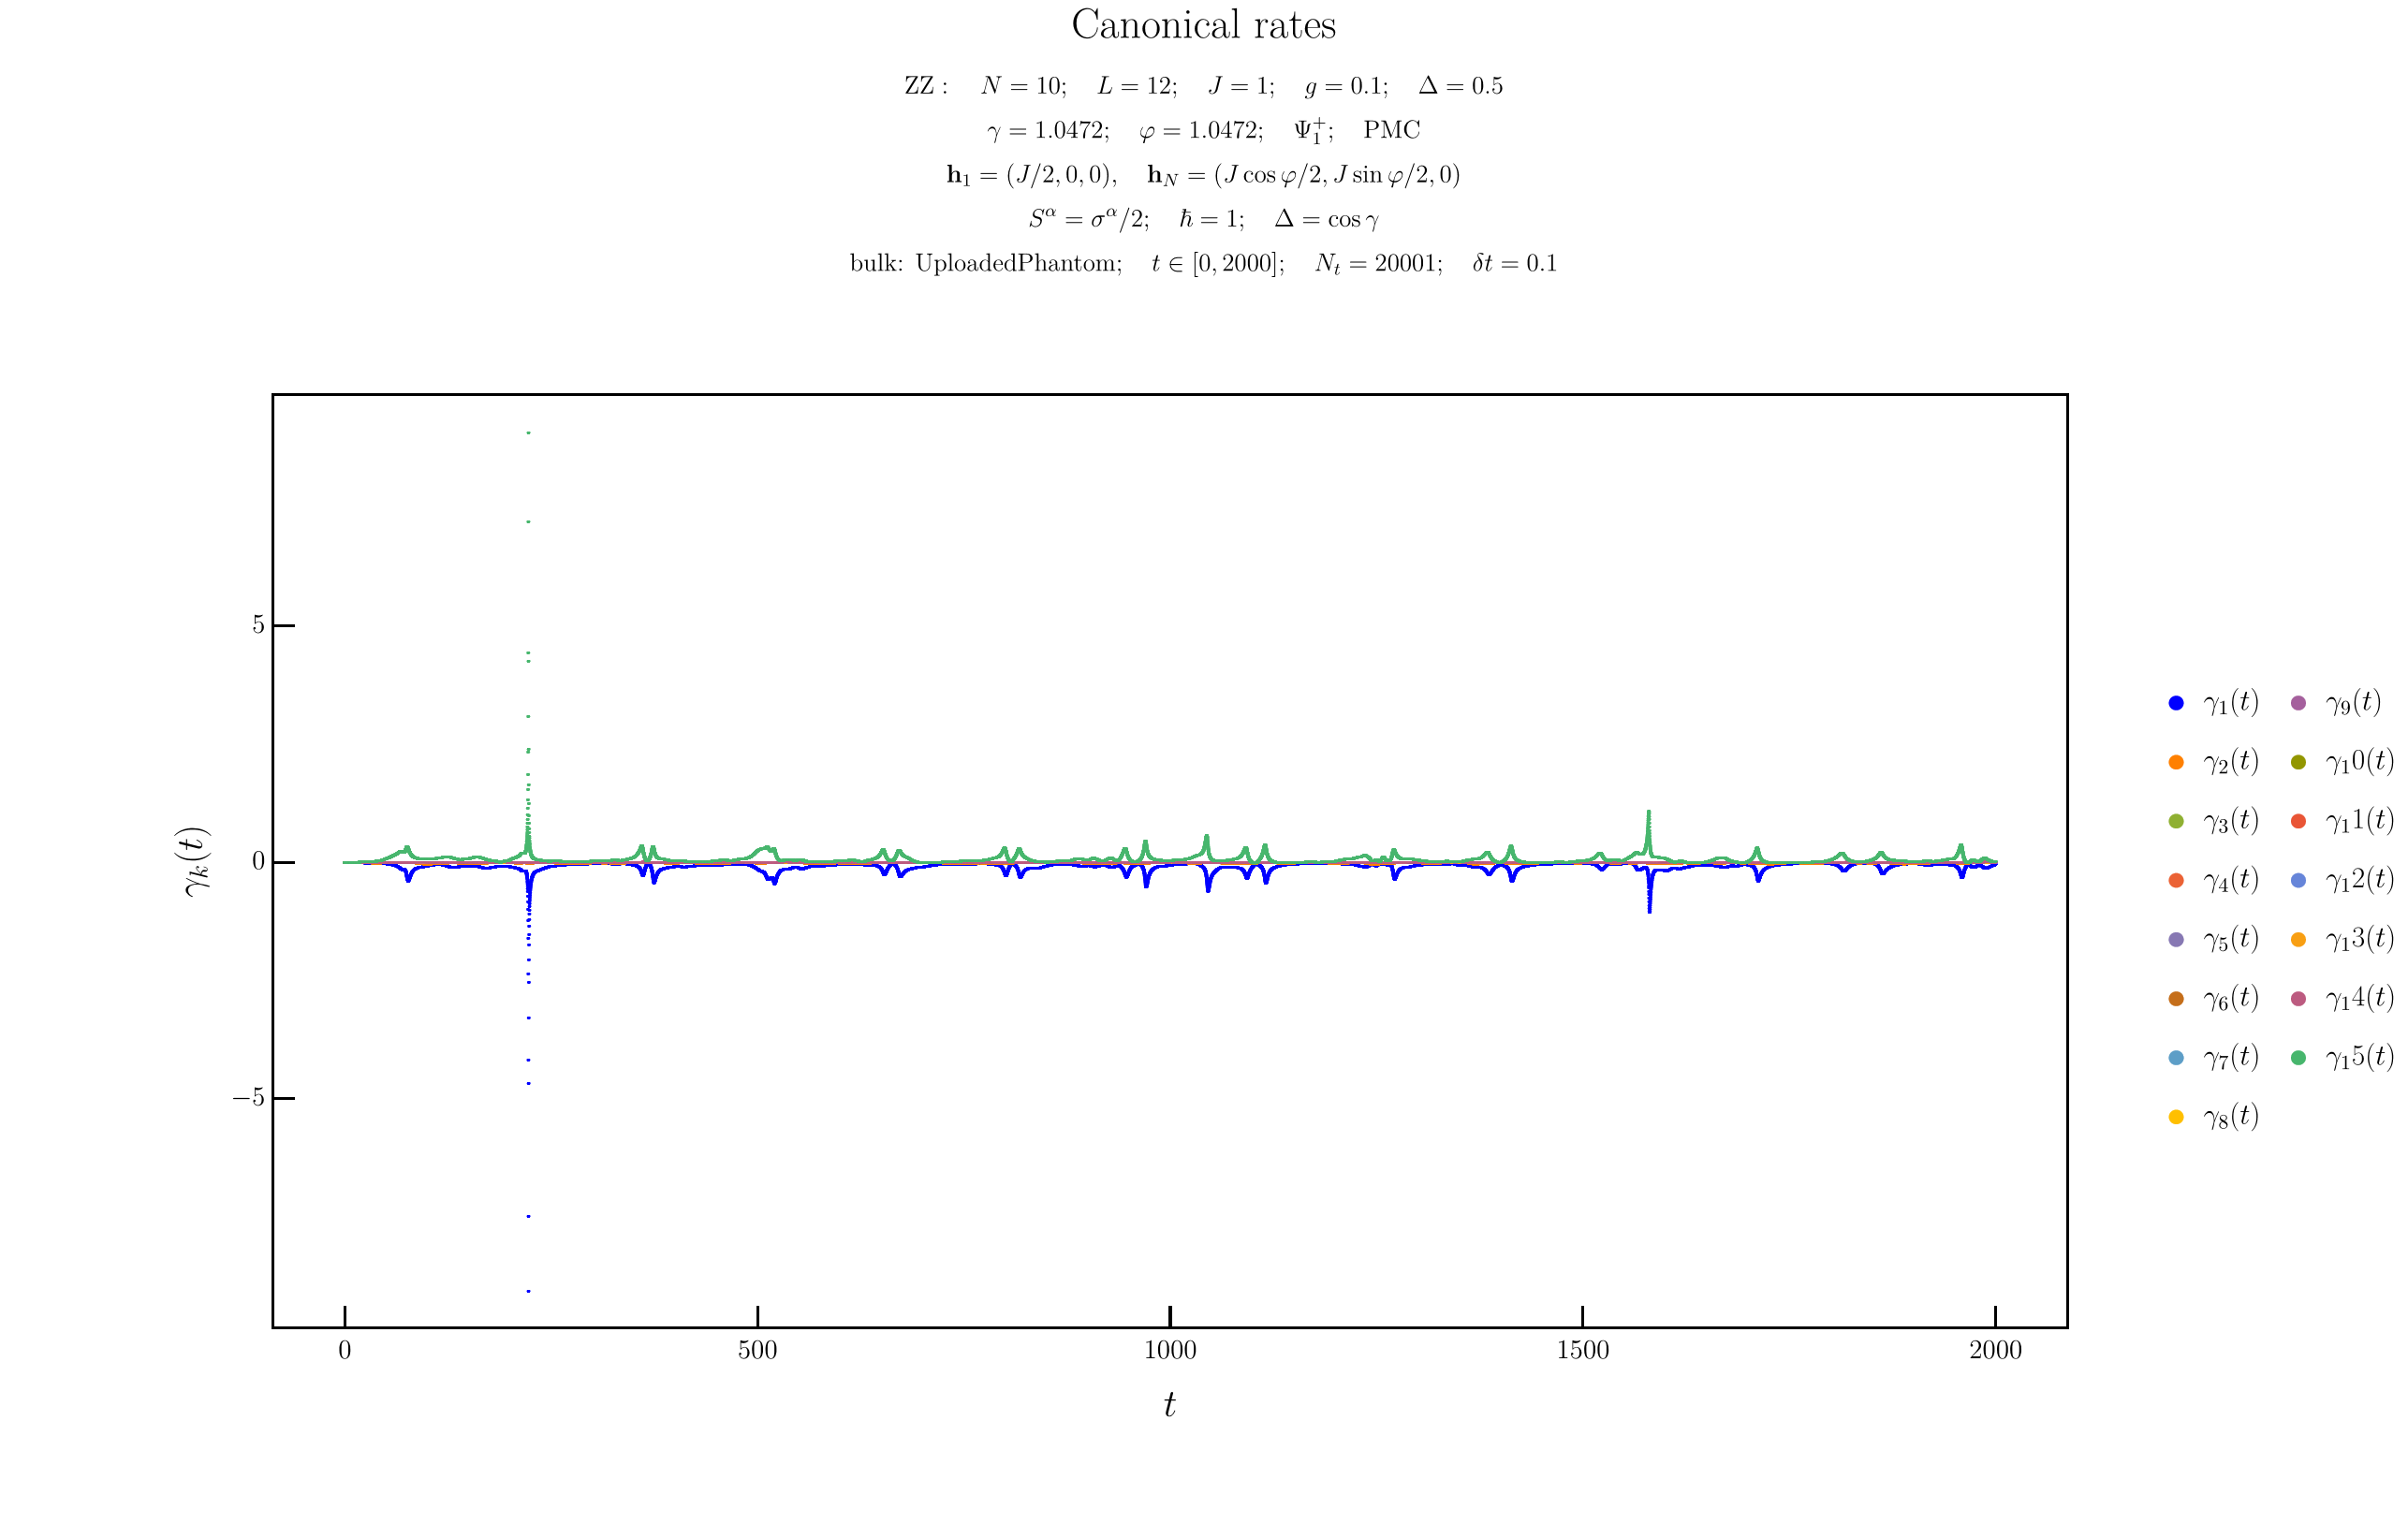
\includegraphics[width=\linewidth,height=0.76\textheight,keepaspectratio]{Channel_CanonicalRates.png}
\end{column}
\begin{column}{0.43\textwidth}
\small
\begin{itemize}\setlength\itemsep{6pt}
\item \textbf{Phantom-helix bulk state} ($\ket{\Psi_1^+}$, $J=1$, $\Delta=\tfrac12$, $g=0.1$, edges in $\ket{++}$): canonical rates show \textbf{large isolated spikes} ($\lvert\gamma\rvert\approx9.7$ at $t\approx223$ for $N=10$, shown; up to $\approx67$ for $N=4$).
\item \textbf{Earlier runs, isolated-chain ground state as bulk state:} the canonical rates stayed small and smooth, with no spikes.
\item Both bulk states are \textbf{pure} and \textbf{eigenstates} of the isolated chain.
\item \textbf{Question:} what property of the initial bulk state separates the two behaviours?
\end{itemize}
\end{column}
\end{columns}
\end{frame}

% ==============================================================
\begin{frame}{Where can large rates come from?}
\small
Write $H_a=H_E+V_a$ with boundary field $V_a=g_As_A^aS_1^z+g_Bs_B^aS_N^z$. For a pure initial bulk state $\ket{\psi_0}$, $\Gamma_{ab}(t)=\langle\phi_b(t)\vert\phi_a(t)\rangle$ with $\ket{\phi_a(t)}=e^{-iH_at}\ket{\psi_0}$, and exact differentiation gives
\[
\frac{\dot\Gamma_{ab}(t)}{\Gamma_{ab}(t)}
=\frac{i\,\bra{\phi_b(t)}(V_b-V_a)\ket{\phi_a(t)}}{\langle\phi_b(t)\mid\phi_a(t)\rangle},\qquad
\lvert\text{numerator}\rvert\le\lVert V_a-V_b\rVert\sim g .
\]
\begin{center}
\fbox{\parbox{0.93\textwidth}{
\begin{itemize}\setlength\itemsep{4pt}
\item The \textbf{numerator} is always small: at most the edge coupling, for \emph{every} bulk state.
\item So the rates can become large \textbf{only if the denominator becomes small}, i.e.\ if two conditional bulk states become (nearly) orthogonal.
\item The question becomes: \textbf{which initial bulk states can a weak boundary field rotate into an orthogonal state?}
\end{itemize}}}
\end{center}
\smallskip
{\color{muted}\footnotesize The same exact identity holds for mixed $\omega_E$, with $\Tr_E[\omega_E U_b(t)^\dagger(\cdots)U_a(t)]$ in place of the overlap.}
\end{frame}

% ==============================================================
\begin{frame}{Hypothesis: degeneracy of the initial bulk level}
\small
\begin{columns}[T,totalwidth=\textwidth]
\begin{column}{0.48\textwidth}
\textbf{Isolated eigenstate}
\begin{itemize}\footnotesize\setlength\itemsep{4pt}
\item The nearest other level (that the boundary field can couple to) is far away compared with the coupling $g$.
\item Mixing those states in costs energy, so the weak field can only slightly deform $\ket{\psi_0}$. Each branch mostly picks up a phase.
\item Conditional bulk states stay nearly parallel, $\lvert\Gamma_{ab}(t)\rvert\approx1$, and the rates stay small.
\end{itemize}
\end{column}
\begin{column}{0.48\textwidth}
\textbf{Eigenstate in a degenerate level}
\begin{itemize}\footnotesize\setlength\itemsep{4pt}
\item Other bulk states sit at the \emph{same} energy.
\item The boundary field can mix them in at \textbf{no energy cost} and rotate $\ket{\psi_0}$ by a large angle inside the level.
\item Opposite edge configurations push in opposite directions ($V_{\bar a}=-V_a$), so conditional bulk states can become nearly orthogonal and the rates spike.
\end{itemize}
\end{column}
\end{columns}
\medskip
\begin{center}
\fbox{\parbox{0.93\textwidth}{\centering
The energy and the magnetization of $\ket{\psi_0}$ do not decide this. What decides it is whether $\ket{\psi_0}$ has degenerate partners that the boundary field connects it to.}}
\end{center}
\smallskip
{\color{muted}\scriptsize
\textbf{Caveats:} (1) \emph{Necessary, not sufficient:} if $\ket{\psi_0}$ is already an eigenvector of the boundary field within the level, it is not rotated and nothing happens.\quad
(2) \emph{Meaning of ``degenerate'':} $V_a$ conserves $M_z$, so only degeneracies within the same $M_z$ sector count; in practice, ``degenerate'' means gap $\lesssim$ coupling.}
\end{frame}

% ==============================================================
\begin{frame}{Simplest example: a two-level bulk}
\begin{columns}[T,totalwidth=\textwidth]
\begin{column}{0.54\textwidth}
\footnotesize
Keep two bulk levels, $H_E=\tfrac{\Delta}{2}\sigma^z$ (splitting $\Delta$), with opposite boundary fields $V_a=+\delta\sigma^x$, $V_{\bar a}=-\delta\sigma^x$, starting in an eigenstate of $H_E$:
\vspace{-6pt}
\[
\Gamma_{a\bar a}(t)=1-2\,\frac{\delta^2}{\Omega^2}\sin^2(\Omega t),\quad
\Omega=\sqrt{\tfrac{\Delta^2}{4}+\delta^2}.
\]
\vspace{-6pt}
\begin{itemize}\setlength\itemsep{1.5pt}
\item \textbf{Gapped ($\Delta\gg\delta$):} $\Gamma_{a\bar a}\approx1$; rates stay small.
\item \textbf{Degenerate ($\Delta=0$):} $\Gamma_{a\bar a}=\cos(2\delta t)$ hits zero periodically; $\kappa=-\tfrac{d}{dt}\ln\lvert\Gamma\rvert$ spikes ($E_0$ drops out).
\item \textbf{Spike height:} if $\ket{\psi_0}$ sits unevenly in the degenerate level, $\lvert\Gamma\rvert$ dips to a small nonzero value and the spike is \textbf{tall but finite}, as in the helix data ($\min\lvert\Gamma_{01,10}\rvert\approx10^{-4}$; exact zeros: Appendix).
\item \textbf{More than two states ($d>2$):} coupling to multiple partners mixes several rotation frequencies, giving \textbf{isolated, irregular spikes} instead of periodic ones (same mechanism).
\end{itemize}
\end{column}
\begin{column}{0.44\textwidth}
\centering
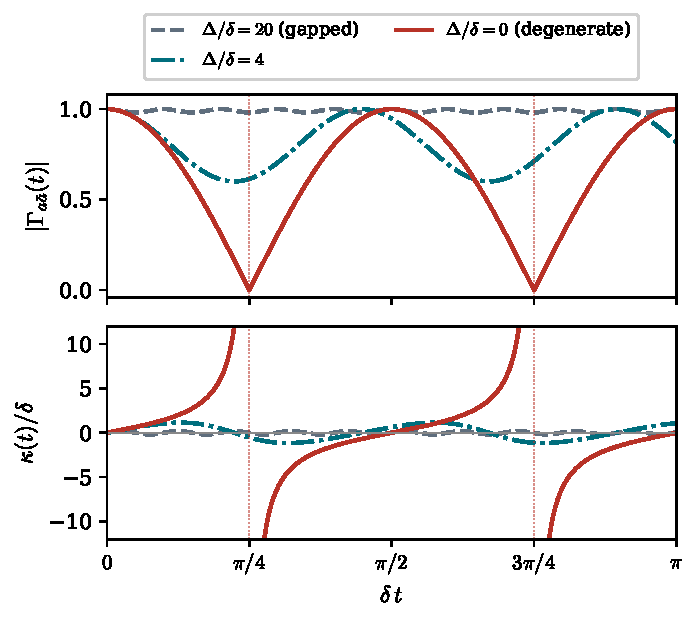
\includegraphics[width=\linewidth,height=0.52\textheight,keepaspectratio]{two_level_bulk.pdf}

{\scriptsize\raggedright
In the $H_E$ eigenbasis $\{\ket{E_+},\ket{E_-}\}$ ($\ket{\psi_0}=\ket{E_+}$, $\delta=\bra{E_+}V_a\ket{E_-}$ from the $z$-field $V_a$, $\bar a$ opposite to $a$):\\[-8pt]
\[
\begin{aligned}
\Gamma_{a\bar a}(t)&=\bra{\psi_0}U_{\bar a}(t)^\dagger U_a(t)\ket{\psi_0}\\[-2pt]
&=\bra{E_+}e^{i(\frac{\Delta}{2}\sigma^z-\delta\sigma^x)t}e^{-i(\frac{\Delta}{2}\sigma^z+\delta\sigma^x)t}\ket{E_+}.
\end{aligned}
\]}
\end{column}
\end{columns}
\end{frame}

% ==============================================================
\begin{frame}{Is the hypothesis consistent with the runs?}
\small
Compare the gap to the nearest coupled bulk level with the boundary-field norm $\lVert V_a\rVert=(g_A+g_B)/4=0.05$ ($J=1$, $g_A=g_B=0.1$, $S^\alpha=\sigma^\alpha/2$):
\smallskip
\begin{center}
\footnotesize
\begin{tabular}{@{}>{\raggedright\arraybackslash}p{4.6cm}cccc@{}}
\toprule
Bulk state & Level degeneracy & Gap to coupled level & $\text{gap}/\lVert V\rVert$ & Spikes? \\\midrule
Isolated-chain ground state, $N=6$--$10$, $\Delta=0.5,1$ & $1$ (in its $M_z$ sector) & $0.33$--$0.56$ & \textbf{7--11} & No\\[4pt]
Phantom helix $\ket{\Psi_1^+}$, $N=4$--$10$, $\Delta=0.5$ & $d=2$--$8$ & $0.002$--$0.13$ & \textbf{0.04--2.7} & Yes\\\bottomrule
\end{tabular}
\end{center}
\smallskip
\begin{itemize}\footnotesize\setlength\itemsep{3.5pt}
\item \textbf{Ground-state runs (no bulk boundary fields):} for odd $N$ the ground space is $2$-fold degenerate ($M_z=\pm\tfrac12$), but $V_a$ conserves $M_z$ and cannot connect the two partners, so the state behaves as isolated ($\lvert\Gamma_{ab}\rvert\ge0.95$, $\lvert\gamma_k\rvert\le0.01$).
\item \textbf{Helix runs ($N=4,5$, $d=2$):} the observed spike spacing ($\approx70$--$76$) matches an estimate of the rotation frequency set by the boundary field inside the doublet (Appendix~A.3).
\end{itemize}
\smallskip
\begin{center}
\fbox{\parbox{0.88\textwidth}{\centering
The two families differ precisely in degeneracy, and the spikes follow the degeneracy.}}
\end{center}
\end{frame}

% ==============================================================
\begin{frame}{Summary and open questions}
\footnotesize
\textbf{Part I:} No edge state with $C<1$---in particular, no product state---reaches $\ket{\Phi^\pm}$ or $\ket{\Psi^\pm}$, for any bulk state.
\smallskip

\textbf{Part II (logical chain):}
\begin{enumerate}\setlength\itemsep{2.5pt}
\item Global unitarity $\implies\Lambda_t$ is CPTP and smooth for every bulk state and every $t$.
\item A canonical master equation needs $\Lambda_t^{-1}$, i.e.\ $\Gamma_{ab}(t)\neq0$.
\item The rates are built from $\dot\Gamma_{ab}/\Gamma_{ab}$, whose numerator is always $\lesssim g$; large rates therefore require near-orthogonal conditional bulk states.
\item \textbf{Hypothesis:} that happens only when the initial bulk state has (nearly) degenerate partners coupled by the boundary field. Isolated eigenstates are protected.
\item \textbf{Consistent with the runs:} isolated-chain ground states ($\text{gap}/\lVert V\rVert\approx7$--$11$) show no spikes; the phantom helix ($d=2$--$8$, $\text{gap}/\lVert V\rVert\lesssim2.7$) does.
\end{enumerate}
\smallskip

\textbf{Open questions (ongoing work):}
\begin{itemize}\setlength\itemsep{2pt}
\item When are the spikes true divergences (exact zeros of $\Gamma_{ab}$) rather than tall finite near-zeros?
\item Quantitative theory for $d>2$.
\item Mixed bulk states over many levels, which can dephase by phase averaging (a different mechanism).
\item Controlled test: compare an isolated and a degenerate eigenstate in the \emph{same} $H_E$ at fixed $N,g$.
\end{itemize}
\end{frame}

% ==============================================================
\begin{frame}[plain]
\end{frame}

% ==============================================================
\appendix
\section{Appendix: derivations and ongoing analysis}
% ==============================================================

\begin{frame}{Appendix: Possible uses of (near-)divergent canonical rates (I)}
\small
\textbf{Direct consequences of $\Gamma_{ab}(t)=\langle\phi_b(t)\vert\phi_a(t)\rangle$:}
\smallskip
\begin{enumerate}\setlength\itemsep{6pt}
\item \textbf{Edge-only spectral probe of the bulk.}
Spikes require $\ket{\psi_0}$ in a (near-)degenerate level coupled by $V_a$, while $1/\lvert\Gamma_{ab}\rvert$ amplifies near-zeros---helping distinguish helix/phantom states from ordinary chain states via edge dynamics alone:
\begin{itemize}\footnotesize\setlength\itemsep{2pt}
\item no spikes $\implies$ isolated level;\quad periodic spikes $\implies$ $d=2$ (spacing $\pi/(2\delta)$ measures the in-level coupling $\delta$);\quad irregular spikes $\implies$ $d>2$.
\end{itemize}
\item \textbf{Sharp witness of non-Markovianity.}
A zero gives $\gamma_{\min}\to-\infty$ just after $t_*$: maximal violation of CP-divisibility and non-invertibility of $\Lambda_t$---a preparation-controlled breakdown of the time-local description while $\Lambda_t$ remains CPTP.
\item \textbf{Times of perfect which-configuration information.}
$\Gamma_{ab}(t_*)=0$ means orthogonal conditional bulk states (perfect bulk record of $a$ vs.\ $b$, zero edge coherence): candidates for bulk readout of the edges, or times to avoid when edge coherence is a resource (cf.\ the protected CZ-like regime of Part~I).
\end{enumerate}
\end{frame}

% ==============================================================
\begin{frame}{Appendix: Possible uses of (near-)divergent canonical rates (II)}
\small
\textbf{More speculative directions:}
\medskip
\begin{enumerate}\setcounter{enumi}{3}\setlength\itemsep{10pt}
\item \textbf{Sensing.}
Near-divergence peak heights scale as $\delta/\lvert c\rvert$, where $c$ is a small weight imbalance of $\ket{\psi_0}$ inside the degenerate level (or the small imaginary offset of $\Gamma_{ab}$).
\begin{itemize}\footnotesize\setlength\itemsep{3pt}
\item Peak heights therefore respond strongly to weak symmetry-breaking perturbations or small detunings from the exact helix condition.
\end{itemize}
\item \textbf{Control.}
In the $d=2$ regime, zeros occur periodically at times set directly by the edge--bulk coupling $\delta$.
\begin{itemize}\footnotesize\setlength\itemsep{3pt}
\item The times at which a chosen pair of edge configurations is completely dephased (or rephased) could be engineered, connecting to dynamical decoupling and dephasing-free subspaces.
\end{itemize}
\end{enumerate}
\end{frame}

\begin{frame}{Appendix: Derivation of the canonical form (I) --- Entrywise $\mathcal L_t$ and diagonal basis}
\small
\textbf{Step 1 --- Time-local generator on matrix units $E_{ab}=\ket a\bra b$ (where $\Gamma_{ab}(t)\ne0$):}
Differentiating $\rho_{ab}(t)=\Gamma_{ab}(t)r_{ab}$ and substituting $r_{ab}=\rho_{ab}(t)/\Gamma_{ab}(t)$ gives
\[
\dot\rho_{ab}(t)=\eta_{ab}(t)\,\rho_{ab}(t),\qquad
\eta_{ab}(t)=\frac{\dot\Gamma_{ab}(t)}{\Gamma_{ab}(t)}=-\kappa_{ab}(t)+i\omega_{ab}(t),
\]
with $\eta_{aa}=0$, $\eta_{ba}=\eta_{ab}^*$, damping rate $\kappa_{ab}=-\tfrac{d}{dt}\ln\lvert\Gamma_{ab}\rvert$, and phase rate $\omega_{ab}=\operatorname{Im}(\dot\Gamma_{ab}/\Gamma_{ab})$.

\textbf{Step 2 --- Restrict the general GKS--Lindblad form to diagonal operators:}
In an orthonormal traceless basis $\{O_j\}_{j=1}^{15}$, any time-local generator has the unique canonical form \cite{Hall2014}
\[
\mathcal L_t(\rho)=-i[\Heff(t),\rho]+\sum_{j,k=1}^{15}\dmat_{jk}(t)\Bigl(O_j\rho O_k^\dagger-\tfrac12\{O_k^\dagger O_j,\rho\}\Bigr).
\]
\emph{Why only diagonal operators appear:} (i) $\mathcal L_t$ commutes with conjugation by every diagonal unitary $D_\theta$, so by uniqueness $\Heff$ is diagonal and $\dmat$ is block-diagonal in the ``charge'' sectors $\{E_{ab}\}_{a\neq b}$ and $\operatorname{span}\{F_\mu\}$; (ii) fixed populations, $\mathcal L_t(E_{bb})=0$, force every jump block $E_{ab}$ to vanish. Hence $\Heff=\sum_ah_aP_a$ ($\sum_ah_a=0$) and $\dmat$ lives on
$F_1=\tfrac12\sigma_A^z\otimes I$, $F_2=\tfrac12I\otimes\sigma_B^z$, $F_3=\tfrac12\sigma_A^z\otimes\sigma_B^z$.

\appref{A.7}
\end{frame}

% ==============================================================
\begin{frame}{Appendix: Derivation of the canonical form (II) --- Closed-form inversion}
\small
\textbf{Step 3 --- Action of the diagonal ansatz on $E_{ab}$:}
With $F_\mu\ket a=g_\mu^a\ket a$ and $\mathbf g^a=(s_A^a,s_B^a,2s_A^as_B^a)$, form the $4\times3$ eigenvalue matrix
\[
G=\frac12\begin{pmatrix}1&1&1\\1&-1&-1\\-1&1&-1\\-1&-1&1\end{pmatrix},\qquad
G^{\mathsf T}G=I_3,\qquad G^{\mathsf T}\mathbf1=0.
\]
Evaluating $\mathcal L_t(E_{ab})=\eta_{ab}E_{ab}$ with the $3\times3$ Hermitian matrix $\dmat=S+iA$ ($S^{\mathsf T}=S$, $A^{\mathsf T}=-A$ real) gives
\[
\eta_{ab}=-i(h_a-h_b)+\mathbf g^{a\mathsf T}\dmat\,\mathbf g^b
-\tfrac12\mathbf g^{a\mathsf T}\dmat\,\mathbf g^a-\tfrac12\mathbf g^{b\mathsf T}\dmat\,\mathbf g^b
\;\Longleftrightarrow\;
\eta=G\dmat G^{\mathsf T}+(-ih-q)\mathbf1^{\mathsf T}+\mathbf1(ih-q)^{\mathsf T},
\]
where $q_a=\tfrac12\mathbf g^{a\mathsf T}S\mathbf g^a$.
\smallskip

\textbf{Step 4 --- Unique inversion (12 real parameters $\leftrightarrow$ 12 real parameters):}
Multiplying by $G^{\mathsf T}(\cdot)G$ annihilates the $\mathbf1$ terms, and summing $\operatorname{Im}\eta_{ab}$ over $b$ isolates $h_a$:
\[
\boxed{\dmat(t)=G^{\mathsf T}\eta(t)\,G,\qquad
h_a(t)=-\tfrac14\textstyle\sum_{b}\operatorname{Im}\eta_{ab}(t),\qquad
\Heff(t)=\textstyle\sum_a h_a(t)P_a.}
\]
\end{frame}

% ==============================================================
\begin{frame}[shrink=4]{Appendix: Canonical master equation and definition of the canonical rates}
\small
\textbf{Step 5 --- Diagonalize the $3\times3$ Hermitian matrix $\dmat(t)=V(t)\diag(\tilde\gamma_1,\tilde\gamma_2,\tilde\gamma_3)V(t)^\dagger$:}
Setting $L_k(t)=\sum_{\mu=1}^3 V_{\mu k}(t)F_\mu$ ($\Tr L_j^\dagger L_k=\delta_{jk}$, diagonal in $\{\ket a\}$) yields the unique canonical master equation \cite{Hall2014}:
\[
\boxed{\dot\rho=-i[\Heff(t),\rho]+\sum_{k=1}^{3}\tilde\gamma_k(t)\Bigl(L_k(t)\rho L_k(t)^\dagger-\tfrac12\{L_k(t)^\dagger L_k(t),\rho\}\Bigr).}
\]
\textbf{Definition of the 15 numerically computed canonical rates $\gamma_1(t)\le\cdots\le\gamma_{15}(t)$:}
\begin{itemize}\setlength\itemsep{3pt}
\item \textbf{Three active eigenvalues + twelve exact zeros:} with entrywise ratio $[\dot\Gamma\oslash\Gamma]_{ab}=\dot\Gamma_{ab}/\Gamma_{ab}$ ($0$ on diagonal), pad the three eigenvalues below with $12$ structural zeros and sort at each $t$:
\[
\bigl\{\tilde\gamma_1(t),\tilde\gamma_2(t),\tilde\gamma_3(t)\bigr\}=\spec\Bigl(G^{\mathsf T}\bigl[\dot\Gamma(t)\oslash\Gamma(t)\bigr]G\Bigr).
\]
\item \textbf{Sign meaning:} because of the padded zeros, $\gamma_1=\min(0,\tilde\gamma_{\min})\le0$ always. Locally CP-divisible iff $\tilde\gamma_{\min}(t)\ge0$ (i.e.\ $\gamma_1=0$); $\gamma_1<0$ witnesses non-Markovianity while $\Lambda_t$ remains CPTP.
\item \textbf{Rayleigh-quotient bound ($\mathbf e_{ab}=(\mathbf g^a-\mathbf g^b)/\sqrt2$):}
$\gamma_{\min}(t)\le\kappa_{ab}(t)=\mathbf e_{ab}^{\mathsf T}\dmat(t)\mathbf e_{ab}\le\gamma_{\max}(t)$.
\end{itemize}
\end{frame}

% ==============================================================
\begin{frame}{Appendix: When do the canonical rates blow up?}
\small
\begin{itemize}\setlength\itemsep{4pt}
\item \textbf{Exact criterion:} the rates are finite at $t$ iff every $\Gamma_{ab}(t)\neq0$. At a zero of order $r$, $\kappa_{ab}\simeq-r/(t-t_*)$, so $\gamma_{\max}\to+\infty$ before $t_*$ and $\gamma_{\min}\to-\infty$ after it, while $\rho_{AB}(t)$ stays smooth. Since $\Gamma_{ab}$ is a finite sum of exponentials with $\Gamma_{ab}(0)=1$, any zeros are isolated (countable).
\item \textbf{Geometric meaning (pure bulk $\ket{\psi_0}$):} with $\ket{\phi_a(t)}=U_a(t)\ket{\psi_0}$ we have $\Gamma_{ab}(t)=\langle\phi_b(t)\mid\phi_a(t)\rangle$, so
\[
\boxed{\text{large rates}\iff\text{conditional bulk states become (nearly) orthogonal.}}
\]
For mixed $\omega_E$ the same holds for the Hilbert--Schmidt vectors $U_a(t)\sqrt{\omega_E}$.
\item \textbf{But exact real-time zeros are special:} a complex $\Gamma_{ab}$ vanishes only if $\operatorname{Re}\Gamma_{ab}=\operatorname{Im}\Gamma_{ab}=0$ \emph{simultaneously}---two conditions on one variable $t$. Generically one gets a \textbf{near-zero} and a \textbf{tall but finite} peak; an exact divergence needs a symmetry of $(H_E,\omega_E)$ that makes $\Gamma_{ab}$ real (up to a known phase).
\end{itemize}
\appref{A.5--A.6}\quad \ongoing
\end{frame}

% ==============================================================
\begin{frame}{Appendix: Finite peaks vs.\ genuine divergences}
\small
\begin{itemize}\setlength\itemsep{6pt}
\item \textbf{Leading-order picture:} $\Gamma_{a\bar a}$ is real and crosses zero $\Rightarrow$ genuine poles of the canonical rates.
\item \textbf{Beyond leading order} (leakage out of $\mathcal D$, second-order level shifts) $\Gamma_{a\bar a}$ generally becomes complex. A zero crossing of the real part is then accompanied by a small imaginary offset $\epsilon$:
\[
\Gamma(t)\simeq v\,(t-t_0)+i\epsilon\ \Longrightarrow\
\kappa(t)=-\frac{\lvert v\rvert^2(t-t_0)}{\lvert v\rvert^2(t-t_0)^2+\epsilon^2},\qquad
\max\lvert\kappa\rvert=\frac{\lvert v\rvert}{2\lvert\epsilon\rvert}.
\]
A tall, finite, antisymmetric peak; the genuine pole is the limit $\epsilon\to0$.
\item \textbf{Which one occurs is a property of the initial bulk state:} if a symmetry of $(H_E,\omega_E)$ keeps $\Gamma_{a\bar a}$ real, zero crossings---and divergences---are robust; otherwise they are lifted to near-zeros. For the complex helix, $\Gamma_{00,11}$ stays real but $\Gamma_{01,10}$ does not.
\end{itemize}
\medskip
\begin{center}
\fbox{\parbox{0.9\textwidth}{\centering
Degenerate initial bulk state $\Rightarrow$ $O(1)$ rotations of the conditional bulk states $\Rightarrow$ near-orthogonality $\Rightarrow$ large canonical-rate peaks, which become genuine divergences only when $\Gamma_{ab}$ vanishes exactly.}}
\end{center}
\appref{A.5--A.6}\quad \ongoing
\end{frame}

% ==============================================================
\begin{frame}[shrink=6]{Appendix A.1: Isolated eigenstate --- rigorous lower bound on $\lvert\Gamma_{ab}\rvert$}
\footnotesize
\textbf{Lemma 1.} Let $H_E\ket{E_0}=E_0\ket{E_0}$ be non-degenerate, $\Delta E=\operatorname{dist}(E_0,\spec H_E\setminus\{E_0\})$, $v_a=\lVert V_a\rVert<\Delta E/2$, $\varepsilon_a=v_a/(\Delta E-v_a)$. Then for all $t$,
\[
\lvert\Gamma_{ab}(t)\rvert\ge\cos\theta_a\cos\theta_b\cos(\theta_a+\theta_b)-\varepsilon_a-\varepsilon_b-\varepsilon_a\varepsilon_b,\qquad \sin\theta_a\le\varepsilon_a .
\]
\textbf{Proof.}
\begin{enumerate}\setlength\itemsep{2pt}
\item By Weyl, $H_a$ has a unique eigenvalue $E_a\in[E_0-v_a,E_0+v_a]$ (eigenvector $\ket{E_0^a}$); all others are $\ge\Delta E-v_a$ from $E_0$.
\item Write $\ket{E_0}=c_a\ket{E_0^a}+\ket{r_a}$, $r_a\perp E_0^a$. Then $(H_a-E_0)\ket{E_0}=c_a(E_a-E_0)\ket{E_0^a}+(H_a-E_0)\ket{r_a}$ (orthogonal terms); the left side is $V_a\ket{E_0}$, of norm $\le v_a$, and $\lVert(H_a-E_0)r_a\rVert\ge(\Delta E-v_a)\lVert r_a\rVert$. So $\lVert r_a\rVert\le\varepsilon_a$.
\item $\ket{\phi_a(t)}=c_ae^{-iE_at}\ket{E_0^a}+e^{-iH_at}\ket{r_a}$; expanding $\langle\phi_b\vert\phi_a\rangle$, the cross terms are bounded by $\varepsilon_a,\varepsilon_b,\varepsilon_a\varepsilon_b$, and $\lvert\langle E_0^b\vert E_0^a\rangle\rvert\ge\cos(\theta_a+\theta_b)$. $\square$
\end{enumerate}
\textbf{Consequence.} For $\varepsilon\lesssim0.3$ ($\Delta E\gtrsim4.3\,\lVert V\rVert$) the bound is positive for all $t$: no zeros, bounded rates. The relevant scale is the gap to the \emph{nearest other level}, not $J$.\\[2pt]
\textbf{Helix runs:} $\lVert V_a\rVert=g/2=0.05$, while the gap from the helix level ($d=\dim\mathcal D$) is
\begin{center}
\begin{tabular}{@{}lccccccc@{}}\toprule
$N$&4&5&6&7&8&9&10\\\midrule
$d$ / gap $\Delta E$&2 / 0.133&2 / 0.098&4 / 0.018&4 / 0.048&4 / 0.0031&8 / 0.0067&8 / 0.0020\\\bottomrule
\end{tabular}
\end{center}
so these runs are never in the isolated weak-coupling regime.\hfill\ongoing
\end{frame}

% ==============================================================
\begin{frame}{Appendix A.2: Degenerate level --- first-order theory and validity (ongoing)}
\footnotesize
Let $H_EP_{\mathcal D}=E_0P_{\mathcal D}$, $\dim\mathcal D=d\ge2$, $Q=1-P_{\mathcal D}$, $\Delta E=$ gap from $E_0$ to $\spec(H_E|_Q)$. Schrieffer--Wolff gives
\[
H_a^{\mathrm{eff}}=E_0+W_a+K_a+O\!\Bigl(\tfrac{\lVert V\rVert^3}{\Delta E^2}\Bigr),\qquad
W_a=PV_aP,\qquad K_a=PV_aQ(E_0-H_E)^{-1}QV_aP .
\]
\begin{itemize}\setlength\itemsep{3pt}
\item \textbf{First order} ($K_a$ and leakage neglected): $W_{\bar a}=-W_a$, hence $[W_a,W_{\bar a}]=0$ and, with $W_a\ket{u_m}=\delta_m\ket{u_m}$,
\[
\Gamma^{(1)}_{a\bar a}(t)=\Tr_{\mathcal D}\bigl[\omega_E\,e^{iH^{\rm eff}_{\bar a}t}e^{-iH^{\rm eff}_at}\bigr]=\Tr_{\mathcal D}[\omega_Ee^{-2iW_at}]=\sum_{m=1}^dp_me^{-2i\delta_mt},\quad p_m=\bra{u_m}\omega_E\ket{u_m}.
\]
\item \textbf{Second order spoils the reduction:} $K_a$ is quadratic in $V_a$, so $K_{\bar a}=K_a$:
\[
H^{\rm eff}_a=E_0+W_a+K_a,\quad H^{\rm eff}_{\bar a}=E_0-W_a+K_a,\quad [H^{\rm eff}_a,H^{\rm eff}_{\bar a}]=2[W_a,K_a]\neq0 .
\]
\item \textbf{Validity:} $\lVert V\rVert\ll\Delta E$ (leakage $\sim\lVert V\rVert/\Delta E$) and $t\ll\Delta E/\lVert V\rVert^2$ (phase error from $K_a$). The plotted window $t\le2000$ exceeds this.
\item \textbf{Helix runs:} $\max_t\lvert\Gamma^{\rm exact}-\Gamma^{(1)}\rvert$ ($t\le100$) is $0.025$--$0.16$ for $(01,10)$ and $0.27$--$0.52$ for $(00,11)$. For $(00,11)$, $W_{00}\equiv0$ on $\mathcal D$, so first order predicts $\Gamma_{00,11}\equiv1$, while the exact value drops to $0.46$--$0.73$.
\end{itemize}
\end{frame}

% ==============================================================
\begin{frame}{Appendix A.3: Two-fold degenerate level ($d=2$, ongoing)}
\footnotesize
Within first order, with $\sigma=\delta_1+\delta_2$ and $\Delta\delta=\delta_1-\delta_2\neq0$:
\[
\Gamma^{(1)}_{a\bar a}(t)=e^{-i\sigma t}\bigl[\cos(\Delta\delta\,t)-i(p_1-p_2)\sin(\Delta\delta\,t)\bigr],\qquad
\lvert\Gamma^{(1)}_{a\bar a}\rvert^2=\cos^2(\Delta\delta\,t)+(p_1-p_2)^2\sin^2(\Delta\delta\,t).
\]
\begin{itemize}\setlength\itemsep{3pt}
\item \textbf{Zeros} iff $p_1=p_2=\tfrac12$, at $t_n=\frac{(2n+1)\pi}{2\lvert\Delta\delta\rvert}$. Near $t_n$ (put $x=\Delta\delta(t-t_n)$, $\tan(\Delta\delta t)=-\cot x$):
\[
\eta^{(1)}_{a\bar a}=-i\sigma-\Delta\delta\tan(\Delta\delta\,t)=\frac1{t-t_n}-i(\delta_1+\delta_2)-\frac{\Delta\delta^2}{3}(t-t_n)+O\bigl((t-t_n)^3\bigr).
\]
\item \textbf{Balanced weights from symmetry.} $\Theta=(\prod_j\sigma_j^x)K$ maps $(S^x,S^y,S^z)\mapsto(S^x,S^y,-S^z)$, so $[\Theta,H_E]=0$ (XXZ bonds and in-plane fields invariant) and $\Theta V_a\Theta^{-1}=-V_a$. Hence $\Theta W_a\Theta^{-1}=-W_a$: eigenvalues pair as $\pm\delta$ with $\ket{u_-}=\Theta\ket{u_+}$. For an equatorial helix $\Theta\ket{\psi_0}=e^{i\chi}\ket{\psi_0}$, so $p_-=\lvert\langle\Theta u_+\vert\Theta\psi_0\rangle\rvert^2=p_+$, $\sigma=0$, and $\Gamma^{(1)}_{a\bar a}=\cos(2\delta t)$.
\item \textbf{Helix runs:} for $(01,10)$, first-order $\delta=0.0224$ ($N=4$) and $0.0208$ ($N=5$) predict a peak spacing $\pi/(2\delta)\approx70.3$ and $75.6$, as observed.
\item \textbf{Caveat:} this exhibits genuine zeros \emph{within first order}; beyond first order only the evenness of A.5 survives for $(01,10)$, and zeros are generically lifted to near-zeros.
\end{itemize}
\end{frame}

% ==============================================================
\begin{frame}{Appendix A.4: Higher degeneracy ($d\ge3$, ongoing)}
\footnotesize
\textbf{Closed polygon.} Phases $\theta_m$ with $\sum_mp_me^{i\theta_m}=0$ exist iff $\max_mp_m\le\tfrac12$. This is \emph{necessary}, but not sufficient, for $\Gamma^{(1)}(t)=\sum_mp_me^{-2i\delta_mt}$ to vanish, since the phases are confined to the line $\theta_m=-2\delta_mt$.
\medskip

\textbf{Proposition.} Let $d\ge3$ and $\{\delta_m-\delta_1\}_{m\ge2}$ be rationally independent.
\begin{enumerate}\setlength\itemsep{2pt}
\item The flow is dense in $\mathbb T^{d-1}$ (Kronecker), so $\inf_t\lvert\Gamma^{(1)}(t)\rvert=0$ iff $\max p_m\le\tfrac12$.
\item The zero set $Z_p\subset\mathbb T^{d-1}$ has codimension $2$. The frequency vectors whose line meets $Z_p$ form a countable union of codimension-1 sets: measure zero.
\item Hence, for almost every set of frequencies, $\Gamma^{(1)}$ never vanishes; it only comes arbitrarily close to $0$ over long times.
\end{enumerate}
\medskip
\textbf{Symmetric case.} With $\Theta$-pairing $\pm\delta_\alpha$ (equal weights $p_\alpha$) and weight $p_0$ on $\delta=0$,
\[
\Gamma^{(1)}=p_0+2\sum_\alpha p_\alpha\cos(2\delta_\alpha t)\in\mathbb R,\qquad \inf_t\Gamma^{(1)}=2p_0-1\ \ (\{\delta_\alpha\}\text{ rationally independent}).
\]
Real sign changes, hence first-order zeros, exist iff $p_0<\tfrac12$ (for $d=2$, $p_0=0$).
\medskip

\textbf{Conclusion.} $d>2$ does \emph{not} remove fine-tuning: without symmetry, exact zeros are measure-zero for every $d$. What $d>2$ changes is the \emph{pattern}: a single-frequency comb becomes quasi-periodic, multi-frequency near-zeros, with only occasional deep dips.
\end{frame}

% ==============================================================
\begin{frame}{Appendix A.5: Exact symmetries of the helix preparation (ongoing)}
\footnotesize
Let $K$ be complex conjugation in the computational basis, $\mathcal R$ the reflection $j\mapsto N+1-j$, $M_z=\sum_jS^z_j$, and
\[
\Theta=\Bigl(\textstyle\prod_j\sigma^x_j\Bigr)K,\qquad T=e^{-i\varphi M_z}\,\mathcal R\,K .
\]
Both commute with $H_E$; $\Theta V_a\Theta^{-1}=V_{\bar a}$; $TS^z_1T^{-1}=S^z_N$; and both fix $\ket{\Psi_1^+}$ up to a phase. (For $T$: in-plane angles map as $\theta_j=\pi+(j-2)\gamma\mapsto\varphi-\theta_{N+1-j}=\theta_j-2\pi$, using $\varphi=(N-3)\gamma$.)
\medskip

\textbf{Proposition 2 (evenness).} $\Gamma_{a\bar a}(t)=\Gamma_{a\bar a}(-t)$.\\
\emph{Proof.} $\Theta U_a(t)\Theta^{-1}=U_{\bar a}(-t)$ and $\langle\Theta x\vert\Theta y\rangle=\langle y\vert x\rangle$, so
$\Gamma_{a\bar a}(t)=\langle U_{\bar a}(t)\psi\vert U_a(t)\psi\rangle=\langle\Theta U_a(t)\psi\vert\Theta U_{\bar a}(t)\psi\rangle=\langle U_{\bar a}(-t)\psi\vert U_a(-t)\psi\rangle$. $\square$
\medskip

\textbf{Proposition 3 (reality of $\Gamma_{00,11}$, for $g_A=g_B$).} $T$ maps $V_a\mapsto V_{\sigma(a)}$, where $\sigma$ swaps $01\leftrightarrow10$. The same steps give $\Gamma_{ab}(t)=\Gamma_{\sigma(b)\sigma(a)}(-t)$. Hence $\Gamma_{00,11}(t)=\Gamma_{11,00}(-t)=\Gamma_{00,11}(-t)^*=\Gamma_{00,11}(t)^*$. For $(01,10)$ this reproduces only Proposition 2. $\square$
\medskip

\textbf{Real bulk preparations.} If $H_E$ is real (no $S^y$ fields) and $\psi_0$ is real, then $K$ itself gives $\Gamma_{ab}(t)^*=\Gamma_{ab}(-t)$; together with $\Theta$, \emph{every} $\Gamma_{a\bar a}$ is real. The complex helix breaks $K$.
\end{frame}

% ==============================================================
\begin{frame}{Appendix A.6: Real zeros and shape of a near-zero (ongoing)}
\footnotesize
\textbf{Real versus complex.} $\Gamma_{ab}$ extends to an entire function of $t$.
\begin{itemize}\setlength\itemsep{2pt}
\item If $\Gamma_{ab}$ is real on the real axis, Schwarz reflection gives $\Gamma_{ab}(\bar t)=\overline{\Gamma_{ab}(t)}$: complex zeros come in pairs $t,\bar t$, which can collide and split along the real axis. Real zeros (sign changes) are \emph{robust}, occupying open regions of parameter space.
\item If $\Gamma_{ab}$ is only even, a simple zero $t_k(\lambda)$ moves analytically with a parameter $\lambda$; a real zero needs $\operatorname{Im}t_k(\lambda)=0$, one real condition: isolated parameter values only. At generic parameters, no real zero.
\end{itemize}
\textbf{Lemma 4 (lifting).} If $\Gamma(t_*)=0$, $\dot\Gamma(t_*)=v\neq0$, and $\Gamma\to\Gamma+\delta\Gamma$ with $\lVert\delta\Gamma\rVert=\epsilon$, then $\min\lvert\Gamma+\delta\Gamma\rvert=\lvert\operatorname{Im}(\bar v\,\delta\Gamma(t_*))\rvert/\lvert v\rvert+O(\epsilon^2)$, nonzero unless $\delta\Gamma(t_*)\parallel v$.
\medskip

\textbf{Near-zero shape.} At closest approach $t_0$, $\Gamma\simeq e^{i\beta}(\lvert v\rvert\tau+i\epsilon')$ with $\tau=t-t_0$:
\[
\kappa=-\frac{\lvert v\rvert^2\tau}{\lvert v\rvert^2\tau^2+\epsilon'^2},\qquad
\omega=-\frac{\lvert v\rvert\epsilon'}{\lvert v\rvert^2\tau^2+\epsilon'^2}.
\]
$\kappa$: bounded antisymmetric peak, extrema $\mp\lvert v\rvert/(2\lvert\epsilon'\rvert)$ at $\tau=\pm\lvert\epsilon'\rvert/\lvert v\rvert$. $\omega$: Lorentzian with area $-\pi\operatorname{sgn}\epsilon'$ (the phase winds smoothly by $\pi$). As $\epsilon'\to0$: $\kappa\to-1/\tau$ and $\omega\to-\pi\operatorname{sgn}(\epsilon')\delta(\tau)$, i.e.\ a genuine pole and a phase jump.
\medskip

\textbf{Helix runs ($t\le2000$):} at the deepest dips $\operatorname{Re}\Gamma_{01,10}\approx0$ while $\operatorname{Im}\Gamma_{01,10}\neq0$, as Lemma 4 predicts; $\min\lvert\Gamma_{01,10}\rvert=5.1\times10^{-4}$ ($N=4$), $1.5\times10^{-2}$ ($N=5$), $1.07\times10^{-4}$ ($N=10$). The resolved peak heights are $66.7$, $2.0$ and $9.7$.
\end{frame}

% ==============================================================
\begin{frame}{Appendix A.7: Why $\Heff$ is diagonal and $\dmat$ lives on $\{F_1,F_2,F_3\}$}
\footnotesize
\textbf{Proposition 7.} Let $\mathcal L_t(E_{ab})=\eta_{ab}E_{ab}$ with $\eta_{aa}=0$, written in Hall's canonical form ($H$ traceless, $\dmat$ Hermitian in an orthonormal traceless basis). Then $H$ is diagonal and $\dmat$ is supported on $\operatorname{span}\{F_1,F_2,F_3\}$.
\medskip

\textbf{Proof.}
\begin{enumerate}\setlength\itemsep{3pt}
\item \emph{Covariance.} For every $D_\theta=\diag(e^{i\theta_a})$, $\mathcal L_t(D_\theta XD_\theta^\dagger)=D_\theta\mathcal L_t(X)D_\theta^\dagger$, since $D_\theta E_{ab}D_\theta^\dagger=e^{i(\theta_a-\theta_b)}E_{ab}$.
\item \emph{Uniqueness transports the data.} $\operatorname{Ad}_{D_\theta^\dagger}\mathcal L_t\operatorname{Ad}_{D_\theta}$ has canonical data $(D_\theta^\dagger HD_\theta,\mathcal C_\theta)$, where $\mathcal C=\sum_{jk}\dmat_{jk}\lvert O_j\rangle\rangle\langle\langle O_k\rvert$ and $\mathcal C_\theta=\operatorname{Ad}_{D_\theta^\dagger}\mathcal C\operatorname{Ad}_{D_\theta}$. By uniqueness, $D_\theta^\dagger HD_\theta=H$ and $\mathcal C_\theta=\mathcal C$ for all $\theta$.
\item \emph{$H$ is diagonal}: the commutant of all $D_\theta$ is the diagonal algebra.
\item \emph{Block structure.} $\operatorname{Ad}_{D_\theta}$ has pairwise distinct characters $e^{i(\theta_a-\theta_b)}$ on $E_{ab}$ ($a\neq b$) and the trivial character on $\operatorname{span}\{F_\mu\}$, so
\[
\mathcal C=\mathcal C_{\rm diag}\oplus\bigoplus_{a\neq b}c_{ab}\lvert E_{ab}\rangle\rangle\langle\langle E_{ab}\rvert .
\]
\item \emph{Fixed populations.} On diagonal $\rho$ the Hamiltonian and $\mathcal C_{\rm diag}$ terms vanish ($F\rho F-\frac12\{F^2,\rho\}=0$), while $D[E_{ab}](E_{bb})=E_{aa}-E_{bb}$. Then $0=\mathcal L_t(E_{bb})=\sum_{a\neq b}c_{ab}(E_{aa}-E_{bb})$, which forces $c_{ab}=0$. $\square$
\end{enumerate}
\end{frame}

% ==============================================================
\begin{frame}{Appendix A.8: Unitary Schur channels cannot entangle on a time interval}
\footnotesize
$\Lambda_t$ is unitary iff $\rank\Gamma(t)=1$, i.e.\ $\Gamma_{ab}=u_au_b^*$, $\lvert u_a\rvert=1$. Then $\diag(u)=e^{i\alpha}(\text{local }z\text{ rotations})\cdot\diag(1,1,1,e^{i\Phi})$ with
\[
\Phi=\arg(u_{00}u_{11}u_{01}^*u_{10}^*),\qquad C\bigl[\Lambda_t(\ket{++}\bra{++})\bigr]=\tfrac12\lvert u_{00}u_{11}-u_{01}u_{10}\rvert=\lvert\sin(\Phi/2)\rvert .
\]
\textbf{Proposition 8.} If $g_A,g_B\neq0$ and $\Lambda_t$ is unitary on an open interval, then $\Lambda_t$ is unitary for all $t$ and $\Phi\equiv0$.
\medskip

\textbf{Proof.}
\begin{enumerate}\setlength\itemsep{3pt}
\item $\lvert\Gamma_{ab}(t)\rvert^2$ is real-analytic; if it equals $1$ on an interval, it equals $1$ everywhere.
\item Let $A_a=U_a\sqrt{\omega_E}$ (Hilbert--Schmidt unit vectors, Gram matrix $\Gamma$). Rank one gives $A_a=u_aM$ with $M=A_{00}$, $u_{00}=1$.
\item From $i\dot A_a=H_aA_a$ and $i\dot M=H_{00}M$: $(V_a-V_{00})M=\lambda_aM$ with $\lambda_a=i\dot u_a/u_a$.
\item $V_{10}-V_{00}=-g_AS^z_1$ and $V_{01}-V_{00}=-g_BS^z_N$, so the range of $M$ lies in joint eigenspaces with $m_1,m_N\in\{\pm\tfrac12\}$; by continuity these values are constant.
\item Then $u_a=\exp\{-it[g_A(s^a_A-\tfrac12)m_1+g_B(s^a_B-\tfrac12)m_N]\}$ is affine in $s_A,s_B$, and the alternating sum in $\Phi$ cancels: $\Phi(t)=\Phi(0)=0$. $\square$
\end{enumerate}
\textbf{Isolated times.} $\rank\Gamma(t_*)=1$ needs all four Gram vectors to realign at once, plus $\Phi=\pi$: many real conditions on one unknown, hence non-generic. Quasi-periodic recurrences return near $\Gamma(0)$ (identity, $\Phi=0$), not to CZ.
\end{frame}

% ==============================================================
\begin{frame}{Appendix A.9: Approximate CZ for an isolated bulk eigenstate}
\footnotesize
Setting of Lemma 1 (A.1), with $\varepsilon\ll1$.
\begin{enumerate}\setlength\itemsep{4pt}
\item \textbf{Near-unitary, uniformly in $t$.} Since $e^{-iH_at}r_a\perp E_0^a$ and $\lvert\langle E_0^b\vert x\rangle\rvert\le\sin\angle(E_0^a,E_0^b)=O(\varepsilon)$ for unit $x\perp E_0^a$, all cross terms are $O(\varepsilon^2)$:
\[
\Gamma_{ab}(t)=u_a(t)u_b(t)^*+O(\varepsilon^2),\qquad u_a(t)=\tfrac{c_a}{\lvert c_a\rvert}e^{-iE_at}.
\]
\item \textbf{Entangling phase.} $\Phi(t)=\Phi_0-J_{\rm eff}t$ with $J_{\rm eff}=E_{00}+E_{11}-E_{01}-E_{10}$ (exact dressed energies). Any function of $s_{A,B}=\pm\tfrac12$ reduces to $\alpha+\beta s_A+\gamma s_B+\delta s_As_B$, and only $\delta$ survives. With $A_n=\bra nS^z_1\ket0$, $B_n=\bra nS^z_N\ket0$:
\[
J_{\rm eff}=g_Ag_B\chi_{1N}+O\!\Bigl(\tfrac{g^4}{\Delta E^3}\Bigr),\qquad
\chi_{1N}=2\operatorname{Re}\sum_{n\neq0}\frac{\bra0S^z_1\ket n\bra nS^z_N\ket0}{E_0-E_n}.
\]
\item \textbf{Fidelity and concurrence.} At $\Phi(t_*)=\pi$, i.e.\ $t_*\simeq\pi/\lvert g_Ag_B\chi_{1N}\rvert\sim\Delta E/g^2$, the fidelity with $\tfrac12\diag(u)\ket{++}$ is $F=\frac1{16}\sum_{ab}u_a^*\Gamma_{ab}u_b=1-O(\varepsilon^2)$; with ``fully entangled fraction $\le(1+C)/2$'', $C\ge2F-1=1-O(\varepsilon^2)$.
\end{enumerate}
\medskip
\textbf{Remarks.} This regime is the opposite of the degenerate helix runs. A thermal $\omega_E$ washes it out (different $J_{\rm eff}$ per eigenstate). The output is $\mathrm{CZ}\ket{++}$, not a computational-basis Bell state.
\end{frame}

% ==============================================================
\begin{frame}{References}
\footnotesize
\nocite{Hall2014,Wootters1998,Parisio2024}
\bibliographystyle{unsrtnat}
\bibliography{references}
\end{frame}

\end{document}
